% mnras_template.tex 
%
% LaTeX template for creating an MNRAS paper
%
% v3.0 released 14 May 2015
% (version numbers match those of mnras.cls)
%
% Copyright (C) Royal Astronomical Society 2015
% Authors:
% Keith T. Smith (Royal Astronomical Society)

% Change log
%
% v3.0 May 2015
%    Renamed to match the new package name
%    Version number matches mnras.cls
%    A few minor tweaks to wording
% v1.0 September 2013
%    Beta testing only - never publicly released
%    First version: a simple (ish) template for creating an MNRAS paper

%%%%%%%%%%%%%%%%%%%%%%%%%%%%%%%%%%%%%%%%%%%%%%%%%%
% Basic setup. Most papers should leave these options alone.
\documentclass[fleqn,usenatbib]{mnras}

% MNRAS is set in Times font. If you don't have this installed (most LaTeX
% installations will be fine) or prefer the old Computer Modern fonts, comment
% out the following line
% Depending on your LaTeX fonts installation, you might get better results with one of these:
%\usepackage{mathptmx}
%\usepackage{txfonts}

% Use vector fonts, so it zooms properly in on-screen viewing software
% Don't change these lines unless you know what you are doing
\usepackage[T1]{fontenc}

% Allow "Thomas van Noord" and "Simon de Laguarde" and alike to be sorted by "N" and "L" etc. in the bibliography.
% Write the name in the bibliography as "\VAN{Noord}{Van}{van} Noord, Thomas"
\DeclareRobustCommand{\VAN}[3]{#2}
\let\VANthebibliography\thebibliography
\def\thebibliography{\DeclareRobustCommand{\VAN}[3]{##3}\VANthebibliography}


%%%%% AUTHORS - PLACE YOUR OWN PACKAGES HERE %%%%%

% Only include extra packages if you really need them. Common packages are:
\usepackage{graphicx}	% Including figure files
\usepackage{amsmath,amssymb}	% Advanced maths commands
\usepackage{multirow}
\usepackage{makecell}
% \usepackage{orcidlink}
\usepackage{physics}
% \usepackage{amssymb}	% Extra maths symbols
\usepackage{newtxtext,newtxmath}

%%%%%%%%%%%%%%%%%%%%%%%%%%%%%%%%%%%%%%%%%%%%%%%%%%

%%%%% AUTHORS - PLACE YOUR OWN COMMANDS HERE %%%%%

% Please keep new commands to a minimum, and use \newcommand not \def to avoid
% overwriting existing commands. Example:
%\newcommand{\pcm}{\,cm$^{-2}$}	% per cm-squared

%%%%%%%%%%%%%%%%%%%%%%%%%%%%%%%%%%%%%%%%%%%%%%%%%%

%%%%%%%%%%%%%%%%%%% TITLE PAGE %%%%%%%%%%%%%%%%%%%

% Title of the paper, and the short title which is used in the headers.
% Keep the title short and informative.
\title[
    \textit{Quasar Island} -- Three new $z\sim$ 6 quasars
]{
    \textit{Quasar Island} -- Three new $z\sim6$ quasars, including a lensed candidate, identified with contrastive learning
}

% The list of authors, and the short list which is used in the headers.
% If you need two or more lines of authors, add an extra line using \newauthor
\author[X. Byrne et\ al.]{
Xander Byrne
% \orcidlink{0000-0001-9488-238X}
$^{1,2}$\thanks{E-mail: ajnb3@cam.ac.uk},
Romain A. Meyer
% \orcidlink{0000-0001-5492-4522}
$^{1,3}$,
Emanuele Paolo Farina
% \orcidlink{0000-0002-6822-2254}
$^{4}$,
Eduardo Ba\~{n}ados
% \orcidlink{0000-0002-2931-7824}
$^{1}$,
\newauthor
Fabian Walter
% \orcidlink{0000-0003-4793-7880}
$^{1}$,
Roberto Decarli
% \orcidlink{0000-0002-2662-8803}
$^{5}$
\\
% List of institutions
$^{1}$Max Planck Institut f\"{u}r Astronomie, K\"{o}nigstuhl 17, D-69117, Heidelberg, Germany\\
$^{2}$Institute of Astronomy, University of Cambridge, Madingley Road, Cambridge, CB3 0HA, UK\\
$^{3}$Department of Astronomy, University of Geneva, Chemin Pegasi 51, 1290 Versoix, Switzerland\\
$^{4}$Gemini Observatory, NSF's NOIRLAB, 670 N A'ohoku Place, Hilo, HI 96720, USA\\
$^{5}$INAF -- Osservatorio di Astrofisica e Scienza dello Spazio di Bologna, Via Gobetti 93/3, 40129 Bologna, Italy
}

% These dates will be filled out by the publisher
\date{Accepted XXX. Received YYY; in original form ZZZ}

% Enter the current year, for the copyright statements etc.
\pubyear{2023}

% Don't change these lines
\begin{document}
\label{firstpage}
\pagerange{\pageref{firstpage}--\pageref{lastpage}}
\maketitle

% Abstract of the paper
\begin{abstract}
Of the hundreds of $z>6$ quasars discovered to date, only one is known to be gravitationally lensed, despite the high lensing optical depth expected at high redshift.
High-$z$ quasars are typically identified in large-scale surveys by applying strict photometric selection criteria, in particular by imposing non-detections in bands blueward of the $\text{Ly}\,\alpha$ line.
Such procedures by design prohibit the discovery of lensed quasars, as the lensing foreground galaxy contaminates the colours of the quasar.
We present a novel quasar selection methodology, applying contrastive learning (an unsupervised machine learning technique) to Dark Energy Survey imaging data.
We describe the training of a neural network which isolates an ``island'' of 11 sources, of which 7 are known high-redshift quasars.
Of the remaining four, three are newly discovered quasars (J0109--5424, $z=6.07$; J0122--4609, $z=5.99$; J0603--3923, $z=5.94$) as confirmed by follow-up Gemini-South/GMOS spectroscopy, implying over 90\% efficiency for our novel selection method.
%% May be updated to all four and 100%!
Detection in the (\textit{g})\textit{r} bands has led these sources to escape selection by traditional colour cuts.
In one case (J0109), emission below the Lyman limit unambiguously indicates the presence of a foreground source, though high-resolution optical/near-infrared imaging is still needed to confirm its lensed (multiply-imaged) nature.
Our findings demonstrate that machine learning techniques can play a key role in unveiling populations of sources missed by traditional methods.
\end{abstract}

% Select between one and six entries from the list of approved keywords.
% Don't make up new ones.
\begin{keywords}
quasars: individual (J0109--5424, J0122--4609, J0603--3923)
%% J0043?
-- quasars: supermassive black holes
-- gravitational lensing: strong
\end{keywords}

%%%%%%%%%%%%%%%%%%%%%%%%%%%%%%%%%%%%%%%%%%%%%%%%%%

%%%%%%%%%%%%%%%%% BODY OF PAPER %%%%%%%%%%%%%%%%%%

\section{Introduction
\label{intro}}


High-redshift ($z\gtrsim6$) quasars are crucial probes of the early Universe, constraining the early growth of supermassive black holes, the properties of the intergalactic medium (IGM), and likely tracing the formation of the first massive structures in the Universe (see e.g.\ \citealt{inayoshi20, volonteri21, fan23} for reviews).

Multi-wavelength large-sky surveys, such as the Dark Energy Survey (DES; \citealt{des}), the VISTA Hemisphere Survey (VHS; \citealt{vhs}), the Wide-field Infrared Survey Explorer (WISE; \citealt{wise}), the Panoramic Survey Telescope and Rapid Response System (Pan-STARRS1; \citealt{panstarrs}) and the Sloan Digital Sky Survey (SDSS; \citealt{sdss}, have enabled the discovery of several hundred high-redshift quasars to date.
Quasars are typically distinguished from other sources, such as stars and galaxies, by their distinctive colour (e.g.\ \citealt{venemans13, banados15, reed15, reed17}).
The high opacity of the neutral IGM at $z>5.5$ creates a distinctive break below the Lyman alpha line, and no flux is expected to be transmitted blueward of the rest-frame Lyman limit ($\lambda=912$\AA; redshifted to $\lambda>6500$\AA).
Hence traditional quasar dropout selection criteria often impose non-detections in the $g$ and $r$ bands \citep{fan01, richards02, reed15, jiang16, Banados2016, reed17, wang19, banados23}.

Such selection criteria are not perfect, and often include contaminants. 
These are most often Galactic brown dwarfs, which have similar colours to high-redshift quasars and are thus difficult to systematically remove \citep{wang19, yang22}.
Moving solar system objects may also contaminate high-redshift quasar searches \citep{bosman23}.
Removing these contaminants requires time-consuming refinement procedures such as visual inspection \citep{venemans13, banados15, reed15} or SED fitting \citep{reed17, andika23}.

Magnification of high-redshift quasars due to gravitational lensing by a massive galaxy on the same line of sight enables the study of quasars of intrinsically lower luminosity, and yields insights into quasars' accretion disks (e.g., \citealt{chan21}) and host galaxies (e.g., \citealt{stacey18}).
Observations of lensed quasars also place constraints on the dark matter profiles in the lensing galaxies (e.g., \citealt{gilman20}), and time-delay cosmography can be used to estimate the Hubble constant independently of the discrepant early- and late-Universe measurements \citep{refsdal64, treu22}.
However, it has long been known that traditional photometric selection criteria exclude lensed high-redshift quasars, as flux from the galaxy can pollute the quasar colour to the extent that it escapes selection (e.g.\ \citealt{wyithe02}, \citealt{pacucci19}).
Indeed, the first (and to date, only confirmed) strongly-lensed $z>6$ quasar to be discovered, J0439+1634 at $z=6.51$, had such a faint lensing galaxy that if the lens were only $0.5\,\text{mag}$ brighter, the quasar would not have met the selection criteria applied \citep{fan19}.

As a result, the fraction of high-redshift quasars observed to be lensed is significantly lower than expected.
The high lensing optical depth at $z>6$ means that the lensed fraction is likely to be higher, with various studies suggesting it should be at least about 1 per cent \citep{yue22} or as high as 20 per cent \citep{pacucci19}.
It is therefore likely that the selection criteria used to identify high-redshift quasars are excluding an entire population.

This paper is not the first attempt to select lensed quasars. \citet{andikaensemble} use an ensemble of state-of-the-art convolutional neural networks (CNNs) trained on mock images to identify 3080 candidate lensed quasars at $z>1.5$ in the Hyper Suprime-Cam Subaru Strategic Survey (HSC-SSP; \citealt{hscssp}), pared down by visual inspection and astrometric information to 210, awaiting spectroscopic confirmation.
At $z\gtrsim6$, \citet{andika23} use a combination of CNNs and SED fitting to identify 448 lensed and unlensed candidate high-redshift quasars in DES, reduced by visual inspection to 36, which also await confirmation.
\citet{yue23} train a probabilistic random forest for their colour selection criteria, followed by morphological selection and a visual inspection phase, discovering an intermediately-lensed (magnified but not multiply-imaged) quasar as well as a quasar pair at $z\sim 5$.
The authors note none the less that the time-consuming visual inspection ``can be replaced by machine-learning-based methods" \citep{yue23}.

The aforementioned works are just two examples of the numerous and varied applications which machine learning (ML) is finding in the natural sciences.
However, the reliance of many popular ML techniques on accurately labelled training data often makes such methods impractical.
In this specific case, the absence of a large training set of real lensed $z\sim6$ quasars is a key weakness of supervised methods.
Unsupervised ML circumvents this necessity by comparing instances to each other and grouping them according to similarity.
In particular, contrastive learning (e.g.\ \citealt{chen20}) seeks a low-dimensional representation of the data by training a CNN to project innocuous transformations (rotations, reflections, etc.) of the same image closer together in a latent space, while aggressively separating projections of different sources.

This paper presents a new contrastive-learning-based methodology to find high-redshift quasars, lensed or not.
We demonstrate the efficiency of this new method in isolating without visual inspection an ``island" of 11 sources, of which at least 10 are quasars.
%% Maybe more! J0043?
This includes three new objects confirmed spectroscopically, which may have been missed by previous searches due to their detections in the \textit{r} band.
In one case, the source is also detected in the \textit{g} band, below the Lyman limit, unambiguously indicating the presence of a foreground source which may be lensing.
This paper is structured as follows. 
In Section \ref{methods} we describe our candidate selection criteria, the contrastive learning approach, and SED fitting of our targets.
Section \ref{confirmation} presents the observations confirming these targets as high-redshift quasars.
Our work is summarized in Section \ref{conc}.

Magnitudes reported in this paper are in the AB system for \textit{g}, \textit{r}, \textit{i}, \textit{z}, \textit{Y}, \textit{J} and \textit{K} bands and the Vega system for \textit{W1} and \textit{W2} bands.
Where required, we use a flat cosmology with $H_0=70\,\text{km}\,\text{s}^{-1}\,\text{Mpc}^{-1}$ and $\Omega_{\mathrm{m}0}=0.3$.


\section{Methods \& Target Selection} \label{methods}

\begin{figure}
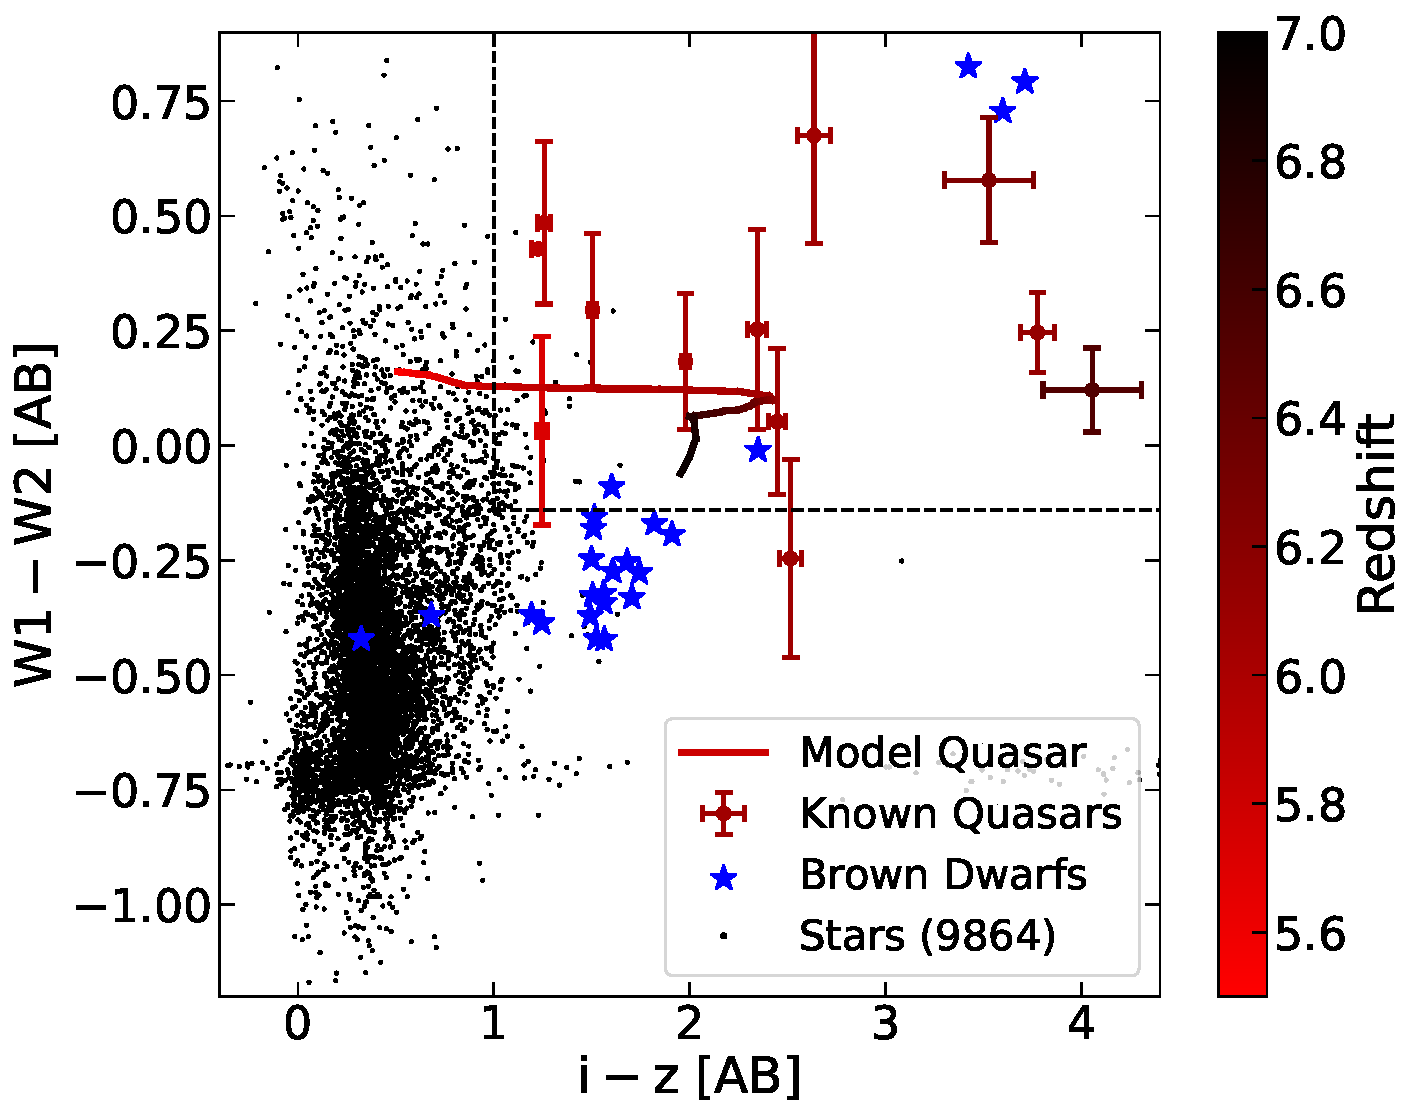
\includegraphics[width=\columnwidth]{figs/selection_criteria.pdf}
\vspace{-.4cm}
\caption{Photometric selection criteria.
The black points are sources selected from three random DES tiles, most of which are likely stars.
The blue stars are brown dwarfs from \citet{kirkpatrick11} and \citet{best15} cross-matched to DES.
Several known high-redshift quasars are plotted, as well as a model quasar track generated using QSOGen \citep{temple22}; both are coloured according to redshift.
Our liberal photometric selection criteria are shown by the dashed lines.
}
\label{fig:colours}
\end{figure}

\subsection{Data preparation} \label{dataprep}

We have used photometric and imaging data from the DES Data Release 2 (DR2), covering 5000 deg$^2$ of the southern celestial hemisphere in the broad \textit{grizY} bands \citep{desdr2}.
The DES DR2 catalogue contains photometry and imagery for almost 700 million objects.
Here we outline the criteria used to select our working sample;
some of these criteria are also shown in Fig.~\ref{fig:colours}.
Our photometric selection criteria are less stringent than in previous studies in order to accommodate lensed quasars, where the lensing galaxy is expected to alter the quasar colour.
All \textit{grizY} magnitudes quoted in this work use the DES DR2 aperture 4, equivalent to $1.95\,\text{arcsec}$ diameter \citep{desdr2}.

We select sources with $\mathit{z} < 21.0$ and $\mathit{Y}<22.45$ to obtain a flux-limited sample; we also impose magnitude errors of $<0.1$ on each of these bands, corresponding to S$/$N$\gtrsim11$.
We further select sources with $\mathit{i}-\mathit{z}>1.0$ to preferentially select quasars and eliminate contaminants such as stars and galaxies, though this is a lower cutoff than in many previous searches (e.g.\ \citealt{reed15, reed17, wang19, Banados2016, banados23}) to allow for photometric contamination from a lensing galaxy.
Unlike most previous works, no requirement is placed on the \textit{g} or \textit{r} bands at this stage.
We apply further standard cuts on the \texttt{IMAFLAGS\_ISO} and \texttt{FLAGS} fields to remove artefacts such as cosmic rays and saturation trails \citep{desdr2}.
The DES DR2 SQL query combining these criteria can be found in Appendix \ref{app_sql}.
These selection criteria result in 218\,241 objects.

We further require a counterpart to each DES source in both VHS DR5 \citep{vhsdr5} and AllWISE \citep{allwise} within $1\,\text{arcsec}$, to remove contaminants as well as artefacts that would be present in only one survey. 
After cross-matching to both surveys, 116\,499 objects remain.
We then use a colour cut of $\mathit{W1}-\mathit{W2}>0.5$ (Vega), to remove a large number of cool dwarf stars, whose \textit{grizY} photometry is often similar to that of high-redshift quasars (e.g.\ \citealt{carnall15}).
After further imposing detection in \textit{J}, \textit{K}, \textit{W1} and \textit{W2} bands, and S$/\text{N}>2$ in all bands, there are 7\,438 objects remaining.

\begin{figure*}
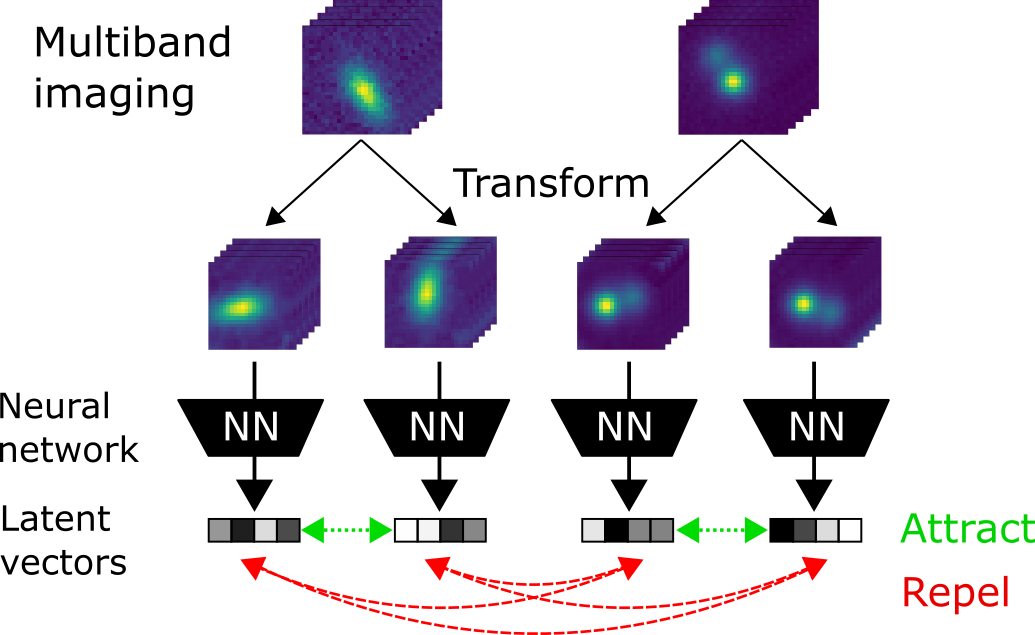
\includegraphics[width=0.8\textwidth]{figs/contrastive.png}
\caption{Schematic of contrastive learning.
The neural network projects transformations of objects in a lower-dimensional latent space.
The contrastive loss function, computed using the proximity of sources in the latent space, rewards proximity between representations of the same source, and penalizes proximity between different sources.
The training procedure is illustrated above for the minimum possible batch size of 2; in practice a larger batch size is used (we use 128, see Table~\ref{tab:hyperparameters}).
The high-dimensional vectors output by the neural network are represented by the shaded sets of 6 boxes; in practice the output dimension is larger (we use 128).
}
\label{fig:contrastive}
\end{figure*}

Despite the large number of remaining objects, no further colour cuts are made, to prevent lensed quasars from being excluded.
Traditional photometric selection criteria are more restrictive, requiring higher thresholds for the $\mathit{i}-\mathit{z}$ colour and making extra cuts on the $\mathit{z}-\mathit{Y}$ or $\mathit{Y}-\mathit{J}$ colours (e.g., \citealt{banados14, Banados2016}).
Stricter criteria naturally lead to a significantly smaller sample size ($\sim 10^2$ objects in the DES--VHS--WISE footprint, e.g.\ \citealt{reed15, reed17}) from which it is not impractical (though potentially unsystematic) to simply inspect the sources individually or run SED-fitting procedures to select good quasar candidates.
However, one of the aims of this work is to dispense with visual inspection altogether.

Furthermore, given the relatively low number density of high-redshift quasars (e.g.\ \citealt{schindler23}) it is likely that our sample of 7\,438 objects is overwhelmingly dominated by contaminants, even taking into account a potentially large fraction of lensed quasars at $z\sim 6$ \citep{pacucci19, minghao22}.
We suggest that it is difficult and perhaps impossible to remove these contaminants by a process based solely on photometry without also removing lensed high-redshift quasars: it is likely that they occupy the same regions of colour space.
Indeed, Fig.~\ref{fig:colours} shows that the $\mathit{i}-\mathit{z}$ and $\mathit{W1}-\mathit{W2}$ colours of high-redshift quasars are shared by brown dwarfs and other objects (likely dusty $z\sim1$ galaxies).

Instead, we suggest that it is possible in principle to distinguish high-redshift quasars from contaminants using source imaging, another data product of DES \citep{des}.
The large number of candidates motivates the use of an ML-based selection, particularly as the application of ML to image classification has rapidly improved in recent years (e.g.\ \citealt{lecun15, pak17}).


\subsection{Contrastive Learning} \label{contrastive}

A requirement of supervised ML techniques is the availability of accurate data labels: poorly-labelled data can severely impede image classification \citep{frenay14}.
Although several known high-redshift quasars are present in our sample, it is \textit{a priori} unknown whether lensed quasars would appear substantially different in DES imaging.
The only known lensed high-redshift quasar (J0439+1634) has been described in detail \citep{fan19}, but is not in the DES footprint.
Additionally, the serendipity of its discovery and its high magnification ($\mu\sim50$) suggest that its appearance could be unrepresentative of the lensed high-redshift quasar population:
magnification distributions are typically taken to be $\sim \mu^{-3}$ \citep{schneider92, wyithe11, minghao22}.
It would therefore be inappropriate to label objects as lensed high-redshift quasars based on subjective similarity to J0439+1634.
In any case, it would be impractical to individually inspect and attempt to label each image in our large sample.

Unsupervised ML techniques do not require data labels, circumventing the above issues.
Not only does this remove the necessity to label each image by hand, it avoids biases due to any prior assumptions about the appearance of lensed quasars in DES imaging.

The novelty in our candidate selection procedure is the use of contrastive learning, an unsupervised ML technique \citep{chen20}.
Briefly, this method trains a neural network to group together similar images in a high-dimensional latent space.
The contrastive loss function used in training rewards proximity in the latent space between projections of transformations of the \textit{same} images, and penalizes proximity of transformations of \textit{different} images.
Over the course of the self-supervised training, similar objects thus end up being clustered together in the latent space.
A schematic of this technique is shown in Fig.~\ref{fig:contrastive} and described below; the training hyperparameters are given in Table~\ref{tab:hyperparameters} in Appendix~\ref{app_contrastive}.

The contrastive learning procedure is as follows.
A batch of $N$ images is selected at random from the data; each ``image" is $28\times28$ pixels ($7.5\times7.5\arcsec$ in DES) in the 5 \textit{grizY} bands, normalized to the brightest pixel across all five bands.
Two sequences of random transformations are then made of each image.
These transformations are such that the classification of the image should not be affected: the image is cropped and may be flipped, rotated, and translated, but the relative brightness of the source in the different bands -- that is, the colour -- is not changed, as this can be a diagnostic feature.
Similarly, the image is not sheared or enlarged in any way, as this could (for example) transform an image of a quasar into an image resembling an extended galaxy.
This transformation stage ensures that the learning process uses only information relevant to source classification, such as colour, shape, extension; not e.g.\ orientation, centering.

These $2N$ transformed images are then each inputted into a CNN, whose architecture is inspired by those of \citet{sarmiento21} and \citet{chen20}, and is given in Table~\ref{tab:architecture} in Appendix~\ref{app_contrastive}.
Contrastive learning CNNs consist of three modules: data augmentation, a base encoder, and a projection head.
The data augmentation module transforms each image as discussed above:
randomly cropping it to $24\times24\times5\,\text{px}$;
randomly flipping it horizontally and/or vertically;
randomly translating it by $2\,\text{px}$;
randomly rotating it.
The base encoder consists of a sequence of three 2D convolutional layers \citep{fukushima79} with exponential linear unit activation \citep{elu}; each layer is followed by a max-pooling layer with pool size 2 \citep{weng92}.
The output of this module is reshaped to a 512-dimensional vector.
Finally, the projection head consists of three densely-connected layers, outputting a vector $\vb*{z}_i$ in a high-dimensional (in this case 128-dimensional) latent space.

The training process consists of altering the weights of the neural network so that similar images are projected to nearby vectors in the latent space, and different images are projected far away from each other.
The contribution of each pair of representations to the loss function is
\begin{equation}
L_{i;j} = -\log \frac{
    \exp(
        \hat{\vb*{z}}_i \cdot \hat{\vb*{z}}_j
        / \tau
    )
}{
    \sum_{k=1, k\neq i}^{2N}
        \exp(
            \hat{\vb*{z}}_i \cdot \hat{\vb*{z}}_k
            / \tau
        )
}
\label{eq:loss}
\end{equation}
where $\hat{\vb*{z}}_i = \vb*{z}_i / \lVert\vb*{z}_i\rVert_\text{L2}$, the vector $\vb*{z}_j$ is that which came from the same original DES object as the vector $\vb*{z}_i$, and $\tau$ is a `temperature' hyperparameter affecting the clustering of the representations.
The loss for a batch is then the average of the above contributions over all $2N$ output vectors.
In minimizing the loss function over multiple batches (and hence transformations), the network thus learns to group together latent vectors from different transformations of the same source, while separating all others.

Following training, the projection head is discarded and the images are inputted directly to the base encoder;
\citet{chen20} showed that removing the projection head improves performance by over 10 per cent.
The output of the encoder is a 512-dimensional vector for each object.
We then apply dimensionality reduction to this set of vectors using $t$-distributed Stochastic Neighbour Embedding ($t$-SNE; \citealt{tSNE}), to be able to visualize the latent space in two dimensions while approximately preserving the distances between the vectors.

\begin{figure*}
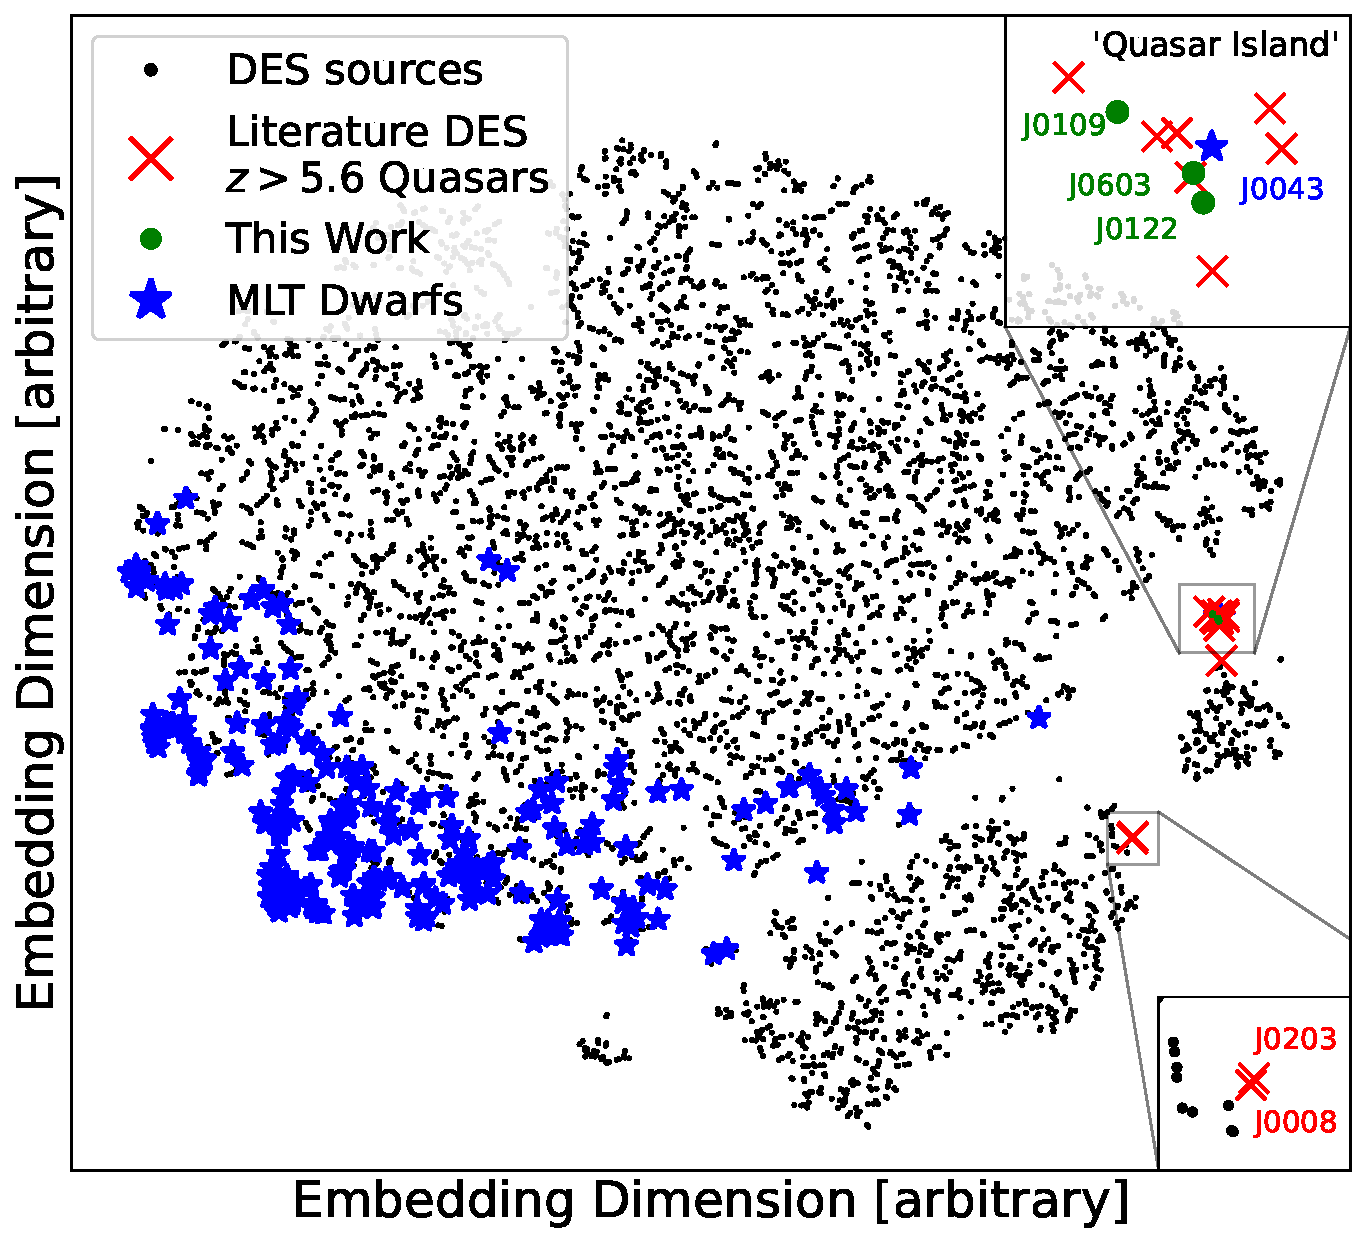
\includegraphics[height=0.4\textheight]{figs/latent_space.pdf}\\
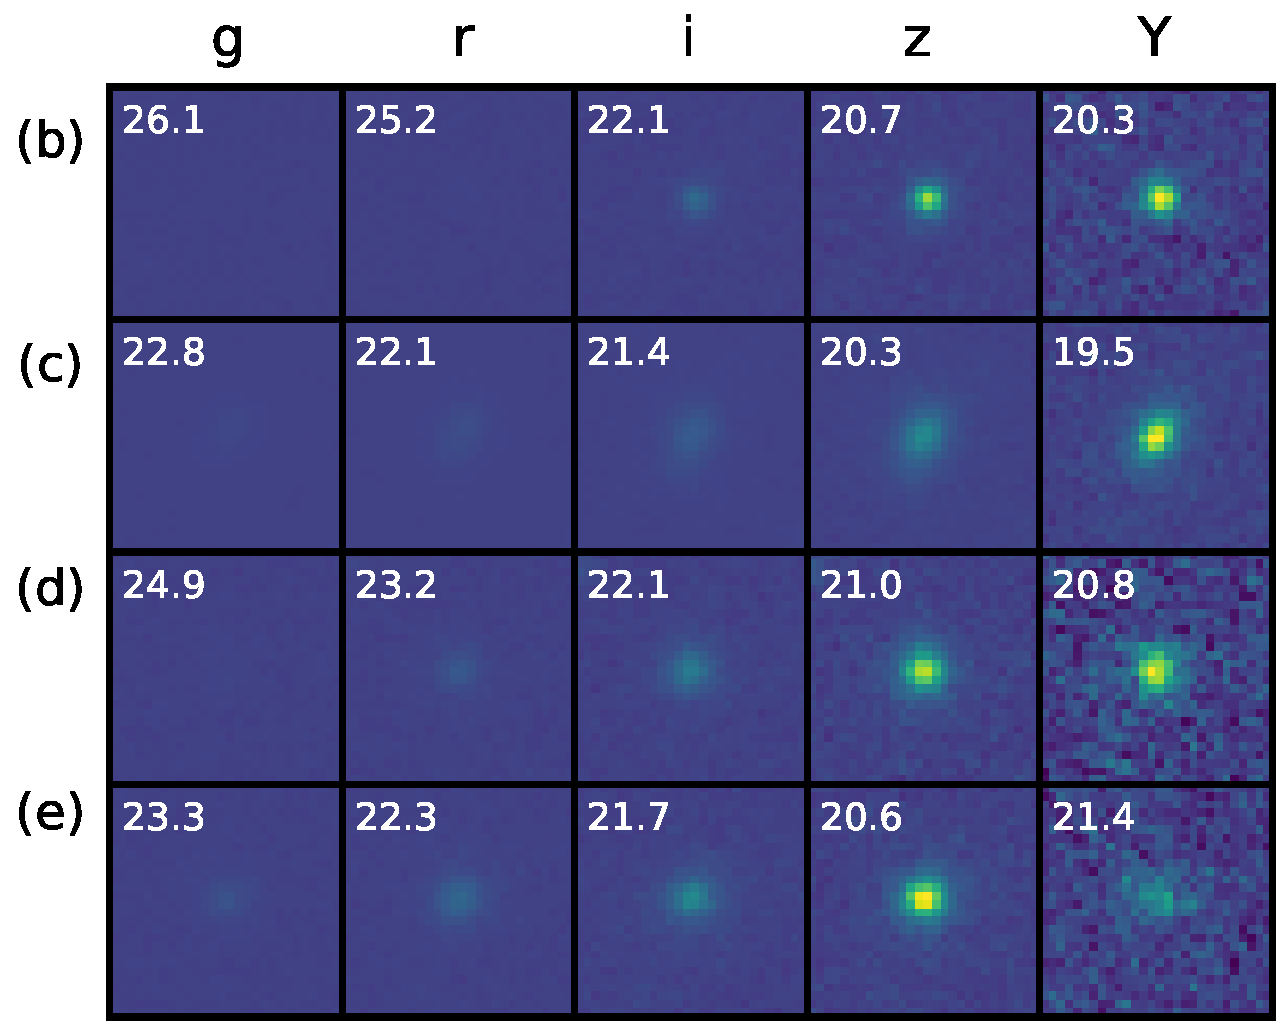
\includegraphics[height=0.5\textheight]{figs/latent_examples.pdf}
\caption{
(a) Dimensionality-reduced projection of DES images.
The known high-redshift quasars were labelled \textit{a posteriori}:
this information was not used in training, yet the neural network has encoded their images together in latent space.
The $t$-SNE procedure reduces the dimensionality of the set of vectors output by the base encoder of the CNN while attempting to preserve the relative distances between each pair of points;
as such the locations of the points would be equally valid if the plot were arbitrarily rescaled or rotated.
There are several distinct groups of objects, including an isolated group containing 11 objects of which 8 are known high-redshift quasars (one of which, J0122, was unpublished).
(b)--(e) DES images of objects sampled from different groups in (a).
}
\label{fig:latent}
\end{figure*}

The result of this dimensionality reduction is shown in Fig.~\ref{fig:latent}(a), separating the sample into several clusters. 
DES images of a member of each is shown in Fig.~\ref{fig:latent}(b)--(e), normalized to the brightest pixel across the five bands.
The largest group contains point sources: most of these objects are likely to be cool dwarfs such as that shown in (b).
Three additional isolated clusters (c--e) contain objects with distinct \textit{grizY} colours.
Their extended morphologies clearly indicate that they are galaxies.
Determining the nature of each of these clusters is beyond the scope of this work.
We note that three peripheral members of groups (d) and (e) are known high-redshift quasars, highlighting the fact that this method does not identify all the quasars in the sample -- and conversely that there may be some unidentified quasars that have been missed by our method.

Finally, an island just above cluster (e) contains 11 objects:
7 known high-redshift quasars;
an unpublished quasar from the ESO archives (J0122--4609, see Section~\ref{archival});
an unidentified object also present in the ESO archives (J0043--6028);
two further sources which had not yet been identified (J0109--5424 and J0603--3923).

Three of these sources (J0109, J0603, J0122) do not meet the traditional colour-cut criteria to be selected as high-redshift quasar candidates as they are detected in the (\textit{g})\textit{r} bands;
we summarise their properties in Table~\ref{tab:threequasars}.
However, their presence in a cluster completely composed by high-redshift quasars suggests them to be so also.
Their detection in the (\textit{g})\textit{r} bands could thus indicate contamination by a foreground lensing object.
The \emph{SEXTRACTOR} \textit{class\_star} probabilities (0: extended source, 1: point-source) for the bluest detected band is $0.32$ and $0.01$ for J0109 and J0603, respectively, further indicating that the contaminating object is a galaxy.
The final source (J0043) has $1800\,\text{s}$ of EFOSC2 spectroscopy in poor weather conditions in the ESO archive (0100.A-0346(A)), but the signal-to-noise ratio is too low to conclude on the nature of this object.
We do not consider this object further.


\begin{table*}
\centering
\caption{
Properties of the three high-redshift quasars identified by our contrastive learning methodology.
Redshifts are obtained spectroscopically.
Upper limits are given at the $2\sigma$ level.
Magnitudes are the DR2 \texttt{MAG\_APER\_4} (see Section~\ref{methods}). The DR2 \textit{class\_star} \textit{SEXTRACTOR} \citep{BertinArnouts96} attributes classify sources between point-like (1) and extended objects (0).
}
\label{tab:threequasars}
\begin{tabular}{cccc}
\hline
& J0122--4609 & J0109--5424 & J0603--3923\\
\hline
R.A.\
& $01^\text{h}22^\text{m}57\fs70$
& $01^\text{h}09^\text{m}09\fs00$
& $06^\text{h}03^\text{m}52\fs26$\\
Dec.\
& $-46\degr09\arcmin14\farcs20$
& $-54\degr24\arcmin16\farcs29$
& $-39\degr23\arcmin35\farcs78$\\
Redshift
& 5.986 & 6.074 & 5.941\\
Spectrum ref.
& 098.A-0439(A) & This work & This work \\
% Photometric Redshift (Q)
% & $5.939\pm0.002$ & $5.999\pm0.002$ & $5.922\pm0.003$ \\
% Photometric Redshift (G+Q)
% & $5.960\pm0.004$ & $6.197\pm0.035$ & $5.939\pm0.006$\\
\textit{g}
&$>26.45$ & $25.07\pm0.15$ & $>26.45$ \\
\textit{r}
& $24.38\pm0.10$ & $23.09\pm0.03$ & $25.34\pm0.19$ \\
\textit{i}
& $21.89\pm0.02$ & $22.73\pm0.04$ & $22.43\pm0.02$ \\
\textit{z}
& $20.09\pm0.01$ & $20.18\pm0.01$ & $20.78\pm0.01$ \\
\textit{Y}
& $20.28\pm0.03$ & $20.19\pm0.03$ & $20.85\pm0.04$ \\
\textit{J}
& $19.73\pm0.18$ & $19.53\pm0.11$ & $20.10\pm0.16$ \\
\textit{K}
& $19.39\pm0.24$ & $19.01\pm0.15$ & $20.08\pm0.42$ \\
\textit{W1}
& $19.40\pm0.08$ & $19.12\pm0.06$ & $19.83\pm0.09$ \\
\textit{W2}
& $19.40\pm0.15$ & $18.72\pm0.08$ & $19.64\pm0.014$ \\
\textit{class\_star\_g} & $0.04$ & $0.32$ & $0.67$ \\
\textit{class\_star\_r} & $0.54$ & $0.82$ & $0.01$ \\
\textit{class\_star\_i} & $0.98$ & $0.95$ & $0.97$ \\
\textit{class\_star\_z} & $0.98$ & $0.98$ & $0.98$ \\
\textit{class\_star\_Y} & $0.93$ & $0.84$ & $0.97$ \\
\hline
\end{tabular}
\end{table*}


\subsection{SED fitting verification} \label{SED}

\begin{table}
\centering
\caption{
Results of SED fitting of the quasar candidates' photometries.
Firstly, using \textsc{LePHARE} \citep{lephare} we find that $\chi^2$ is lowest for a quasar template in both cases.
Secondly, with three sets of templates based on \textsc{BAGPIPES} galaxy models \citep{carnall18} and \textsc{QSOGEN} quasar models \citep{temple22}, we find that the BIC is lowest for a galaxy+quasar model in the case of J0109-5424, but pure quasar models are more suitable for J0603-3923 and J0122-4609.
There is no significance to some values of the BIC being negative.
}
\label{tab:fits}

\begin{tabular}{ccccc}
\hline
Fitting (metric) & Template
& J0109 & J0603 & J0122\\
\hline
\multirow{3}{*}{\makecell{
\textsc{LePHARE}\\($\chi^2$)
}}
& Galaxy & 3913 & 1888 & 3933\\
& Quasar & \textbf{484} & \textbf{20} & \textbf{51}\\
& Star & 3209 & 687 & 1694\\
\hline
\multirow{3}{*}{\makecell{
    \textsc{BAGPIPES}+\\
    QSO templates\\
    (BIC)
}}
& Galaxy & 3676 & 1469 & 3494\\
& Quasar & $-33$ & \textbf{33} & \textbf{79}\\
& Galaxy+Quasar & $\mathbf{-191}$ & 41 & 91 \\
\hline
\end{tabular}
\end{table}

We now investigate further the nature of the two new high-redshift candidates, as well as the archival quasar J0122, using an array of traditional SED fitting codes as well as a custom lensed quasar fit.

As cool dwarfs are expected to constitute the majority of the sample, and several high-redshift quasars were misclassified as brown dwarfs by the neural network, we first compare best-fitting templates of stars and quasars to the photometry of the three objects using \textsc{LePHARE} \citep{lephare}.
The $\chi^2$ of the best-fitting star, galaxy and quasar templates in \textsc{LePHARE} is given in Table~\ref{tab:fits} and their spectra are shown in Fig.~\ref{fig:fits}.
In each case, the $\chi^2$ is much lower ($\Delta\chi^2>600$) for the best-fitting quasar template than the best-fitting star or galaxy template, suggesting that these sources are unlikely to be cool dwarfs or galaxies.

To indicate whether these sources could be lensed, we also performed SED fitting directly to templates of galaxies, quasars and lensed quasars.
This fitting was performed with a custom code making use of the \textsc{emcee} Python package \citep{emcee} to minimize the $\chi^2$ statistic in each case.
The galaxy models were constant-star-formation-rate models from the \textsc{BAGPIPES} package \citep{carnall18}, parametrized by stellar mass, start and end times of the constant star formation, metallicity, redshift, and dust extinction. 
The quasar templates were generated using \textsc{QSOGEN} \citep{temple22}, parametrised using a flux-free scaling factor and colour excess $E_{B-V}$.
Finally, we create simple `galaxy+quasar' composite templates by adding the galaxy templates to the \textsc{QSOGEN} templates, in order to mimic to first order the expected spectrum of a lensed quasar system.

The best-fitting spectra for these three templates are shown in the bottom panels of Fig.~\ref{fig:fits}.
The galaxy templates have 6 free parameters; the quasar templates 2; the lensed quasar templates 8.
To quantify goodness of fit for models with different numbers of fitting parameters, we use the Bayesian information criterion (BIC; \citealt{schwarz78}), which penalizes models with more parameters to discourage overfitting.
The BICs for each model and candidate are also given in Table~\ref{tab:fits}.
For J0109, we find that a galaxy+quasar model is a significantly better model than a pure quasar model by $\Delta\text{BIC}>150$.
The lower left panel of Figure~\ref{fig:fits} shows that the inclusion of galaxy flux in the modelling adds sufficient flexibility to fit the significant flux measured in the \textit{g} band.
For the other two objects, the best-fitting galaxy+quasar model is essentially identical to the best-fitting quasar model: the galaxies in these models contribute very little to all bands.
Table~\ref{tab:fits} shows that J0603 and J0122 have a higher BIC for galaxy+quasar models than quasar models, hence we consider these objects as unlensed quasars.

\begin{figure*}
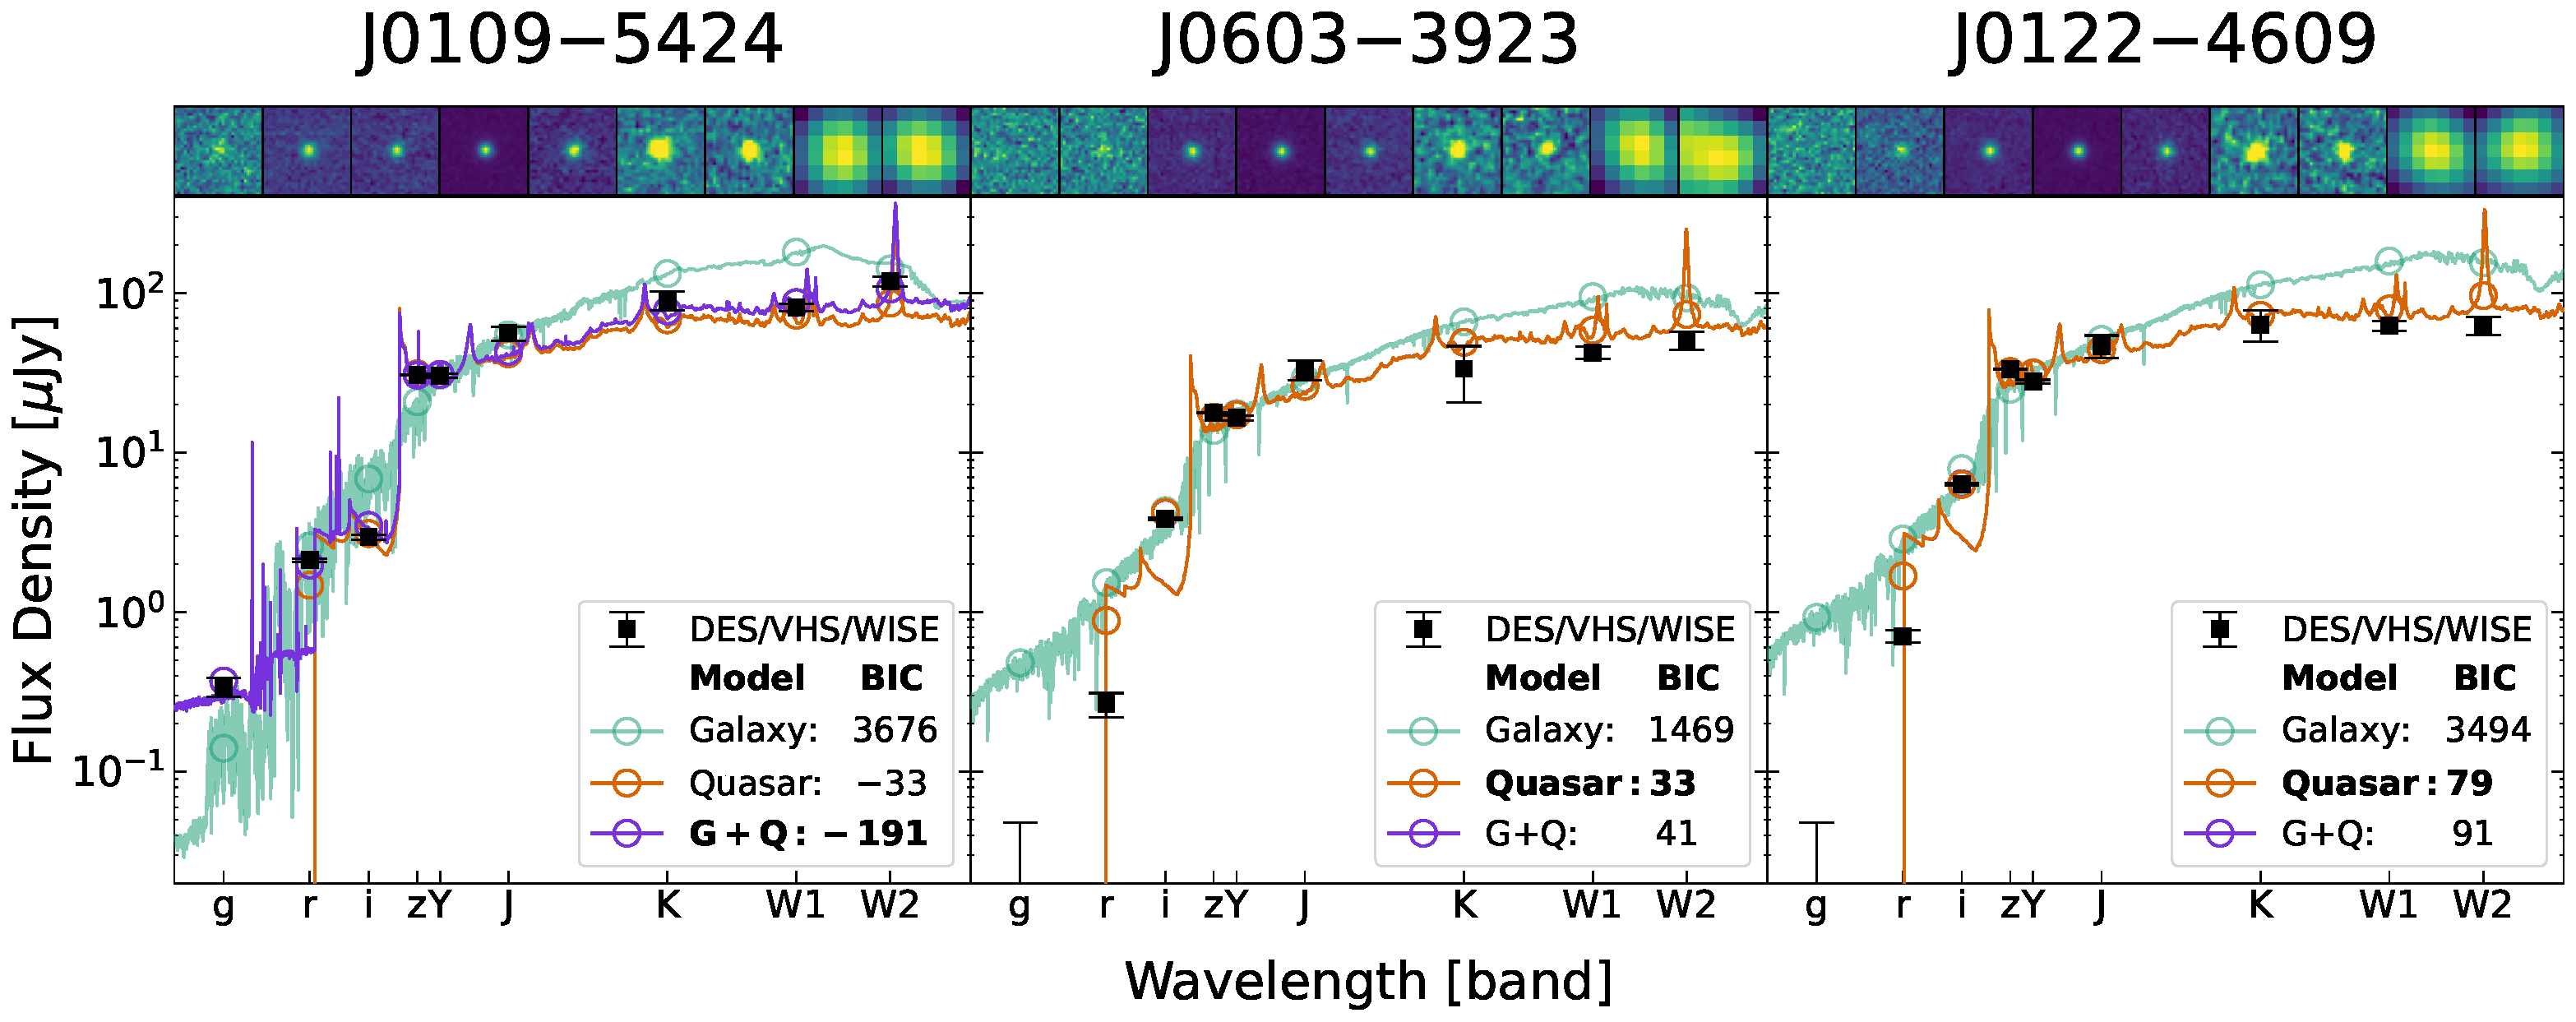
\includegraphics[width=\textwidth]{figs/seds.pdf}
\caption{
DES+VHS+WISE imaging and best-fitting spectra of the candidates' photometry for star, galaxy and quasar templates from \textsc{LePHARE} \citep{lephare}, and galaxy, quasar and lensed quasar templates based on \textsc{BAGPIPES} galaxy models \citep{carnall18} and \textsc{QSOGEN} quasar models \citep{temple22} as described in the text.
Integrated fluxes for \textit{grizY}, \textit{J}, \textit{K}, \textit{W1} and \textit{W2} bands are indicated in the coloured circles.
The observed fluxes measured by the three surveys are indicated by the black squares with error bars.
The bandpass forms are shown at the bottom of each plot.
For J0603 and J0122, the best-fitting galaxy+quasar models are almost identical to the best-fitting quasar models.
}
\label{fig:fits}
\end{figure*}

\section{Follow-up confirmation and archival search} \label{confirmation}

\subsection{An archival \texorpdfstring{$z\sim 6$}{TEXT} quasar: J0122--4609}
\label{archival}
We cross-matched the three unconfirmed candidates with the ESO archive and Gemini-South archive. We found that J0122--4609 had unpublished EFOSC2/NTT spectroscopy (programme 098.A-0439(A)).
It was observed for $1200$s using the $1.0\,\text{arcsec}$-wide slit with grism $\#16$ and the OG530 blocking filter. The spectrum was reduced using \textsc{Pypeit} \citep{pypeit:joss_pub} using the associated bias, flats and standard returned by the ESO archive.
The spectrum clearly shows the Lyman-break and blue UV colors of a high-redshift quasar (see Fig.~\ref{fig:spectra_archival}), confirming the efficiency of our contrastive network to select high-redshift quasars.

\begin{figure}
    \centering
    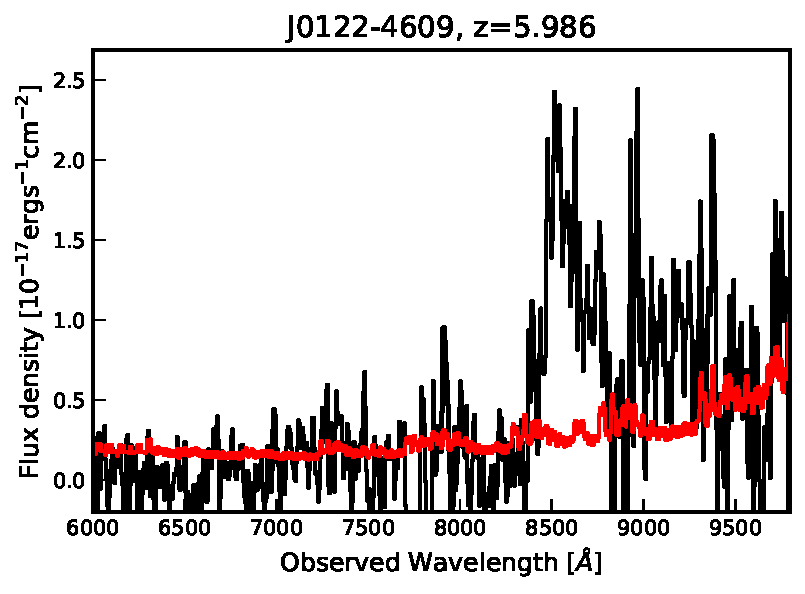
\includegraphics[width=0.48\textwidth]{figs/J0122-4609_1Dspec.pdf} 
    \caption{EFOSC2/NTT spectra of the unpublished quasar J0122--4609 selected by the contrastive network.
    The observed flux density is shown in black, with the error array in red.}
    \label{fig:spectra_archival}
\end{figure}

\subsection{Discovery of two new quasars at \texorpdfstring{$z\sim 6$}{TEXT}, including a lensed candidate}

\begin{figure}
    \centering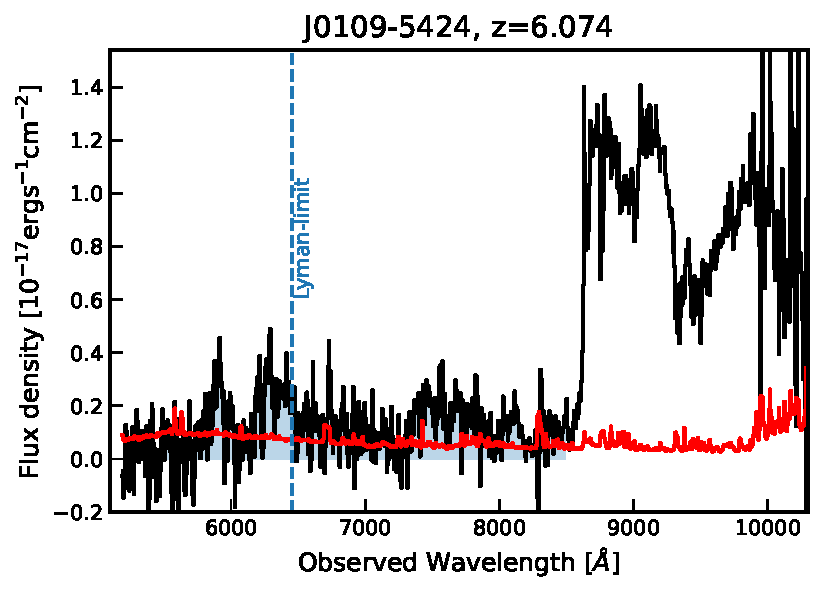
\includegraphics[width=0.48\textwidth]{figs/J0109-5424_1Dspec.pdf} \\
    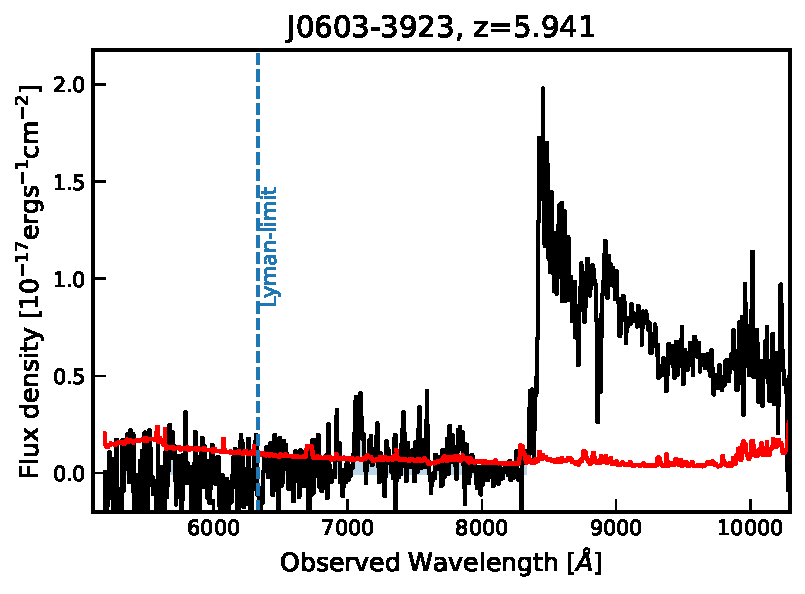
\includegraphics[width=0.48\textwidth]{figs/J0603-3923_1Dspec.pdf} 
    \caption{GMOS-South confirmation spectra of the two lensed quasar candidates presented in this work. The observed flux density is shown in black, with the error array in red. We highlight the presence of residual flux in the Lyman-$\alpha$ forest in light shaded blue and the redshifted Lyman-limit with a vertical dashed line.}
    \label{fig:spectra_gemini}
\end{figure}

The remaining two candidates in the quasar cluster were observed in December 2022 with the Gemini Multi-Object Spectrograph (GMOS) South (Programme ID GS-2022B-FT-208, PI: Farina).
The two candidates were observed in long-slit mode for $4\times300\,\text{s}$ exposures using the $1.5\,\text{arcsec}$ slit width.
We used the R400+G5325 grating in combination with the GG455\_G0329 blocking filter to cover the wavelength range $5300\,\text{\AA}\leq \lambda \leq 10300\,\text{\AA}$ where the Lyman break of a $z\sim 6$ quasar would be expected.
As with J0122 above, the spectra were reduced using \textsc{Pypeit} \citep{pypeit:joss_pub}.

We show the optical GMOS spectra of the two candidates in Fig.~\ref{fig:spectra_gemini}. Both J0109--5424 and J0603--3923 are detected in the $(g),r$ bands, which would lead them to be discarded as contaminants in traditional colour-cut searches. However, the GMOS spectra confirm their quasar nature, validating the efficiency of our contrastive network to find lensed quasar candidates.
Whilst the Lyman-$\alpha$ line and redwards continuum of J0603--3923 is typical of high-redshift quasars, J0109--5424 presents strong BAL features and weak Lyman-$\alpha$ emission.
We fit J0603--3923 with the `median' quasar template of \citet{Banados2016} and J0109--5424 with the `weak' template, deriving best-fitting redshifts of $z=5.941$ and $6.074$, respectively.
The error of these templates compared to the \ion{Mg}{ii} or [\ion{C}{ii}] redshifts is typically $\sigma(\Delta z<0.03)$ \citep{banados23}.

% The spectroscopic redshifts are in relatively good agreement with the photometric redshifts derived with our simple composite quasar+galaxy templates described in Section \ref{SED}. For J0603--3923 we find $z_{\rm{phot}}=5.94$, whereas we find a larger redshift for J0109--5424 ($z_{\rm{phot}}=6.20$) which could be explained by the simplistic modelling of the galaxy spectrum and/or the strong BAL features not present in the \citet{vandenberk01} template.

Interestingly, the spectrum of J0109--5424 presents significant flux throughout the Lyman-$\alpha$ forest and even below the Lyman-limit.
This is an unambiguous signature of a foreground, potentially lensing, galaxy contaminating the photometry of the quasar, making J0109--5424 the first lensed BAL quasar candidate at high-redshift.
The lensed nature of J0603--3923 is more uncertain as we do not detect flux below the Lyman limit.

Another argument for the lensed nature of the two objects is their extremely short proximity zones.
Using the standard definition of the ionized near-zone \citep{Eilers2021}, we measure $r_\text{NZ}= 0.41 \pm 0.12(1.15) \rm{Mpc}$ for J0109--5424 and $r_\text{NZ} = 3.6 \pm 0.12 (1.21) \rm{Mpc}$ for J0603--3923, where the first error is due to the resolution of the GMOS spectra and the second stems from the uncertainty of the quasar redshift.
The expected proximity zones for J0109--5424 ($M_{1450} = -25.18$) and J0603--3923 ($M_{1450} = -25.73$) are $r_\text{NZ}\simeq 3 \rm{Mpc}$ \citep{Eilers2017}, although considerable scatter exists in the $z=6$ quasar population \citep{Eilers2021,Satyavolu2023}, consistent with the measurement for J0603--3923.
However, the near-zone of J0109--5424 is much smaller than expected, and is more common for quasars with $M_{1450} \simeq -23$, strongly arguing for this object to be gravitationally lensed and magnified (see e.g. \citealt{Davies2020}).
ALMA [\ion{C}{ii}] 158 $\mu \rm{m}$ redshifts are needed to improve the proximity zone measurement, as well as space-based high-resolution imaging to definitely confirm their lensed nature. 

In summary, multiple arguments point to a lensed nature for J0109-5424: the SED modelling, the detection of flux below the Lyman limit and the near-zone size. Confirming the lensed nature of J0109 would significantly increase the observed lensed fraction of $z\sim 6$ quasars.
The DES--VHS--WISE detected sources sample we have used in this work contains $13$ $z\sim6$ quasars (see Section \ref{contrastive}), of which one is a lensed quasar candidate.
This would imply an observed lensed fraction of $7.7_{-4.7}^{+10.8}$ per cent.
This is consistent with both \citet{pacucci19} who predict a $z\sim 6$ lensed fraction between $6$ and $20$ per cent, and \citet{minghao22} who give a revised estimate using more recent lens parameters at $1$--$6$ per cent depending on the bright-end slope of the $z\sim 6$ quasar luminosity function. 

\section{Conclusions} \label{conc}

We have developed a novel methodology based on unsupervised machine learning to find high-redshift quasars that have been missed by previous surveys, including gravitationally-lensed objects.
This new method, relying on relaxed colour cuts and the use of DES imaging data, is completely automated and does not require any visual inspection.
Our method isolated 11 objects in the DES--VHS--WISE footprint, at least 10 of which are high-redshift quasars.
Of these, we report the discovery of two, and publish another from the ESO/Gemini-South archive.
One of the newly-discovered quasars, J0109--5424, is likely lensed: it is detected in the \textit{gr} bands and its spectrum shows significant flux in the Lyman-$\alpha$ forest and even below the Lyman limit.
Detections in the \textit{gr} bands had likely caused this quasar, as well as J6003--3923 in the \textit{r} band, to be missed by previous searches, which excluded objects with such photometric detections to avoid contamination by cool dwarfs.
Follow-up high-resolution imaging is now needed to confirm the lensed nature of J0109, which would make it the second lensed high-redshift quasar to be discovered.

The discovery of a lensed high-redshift quasar in the DES footprint would suggest that a significant fraction of the high-redshift quasar population has been missed due to the photometric contamination induced by lensing galaxies.
The magnification effect induced by gravitational lensing brings ever fainter quasars into view, and this work suggests that lensed high-redshift quasars are not as uncommon as the paucity of the known population would suggest.
As such it is likely that lensed quasars will be observed deeper into the epoch of reionization, opening up new avenues with which to probe the high-redshift Universe.


\section*{Acknowledgements}

This research made use of the cross-match service provided by CDS, Strasbourg \citep{boch12} and the \textsc{Astropy} Python package \citep{astropy1, astropy2, astropy3}.
XB thank the Max Planck Institute for Astronomy, for the funding of the internship within which this work was conducted. RAM, FW acknowledge support from the ERC Advanced Grant 740246 (Cosmic\_Gas). RAM acknowledge support from the Swiss National Science Foundation (SNSF) through project grant 200020\_207349.

%%%%%%%%%%%%%%%%%%%%%%%%%%%%%%%%%%%%%%%%%%%%%%%%%%
\section*{Data Availability}

The DES photometric and imaging data used in this work are publicly available at \url{https://www.darkenergysurvey.org/the-des-project/data-access/}.
The contrastive network architecture and trained weights will be made available upon acceptance of the manuscript at \url{https://github.com/xbyrne/glq_mpia}.
The archival spectrum presented in this work is available in the ESO archive (Proposal ID: 098.A-0439(A)). 


%%%%%%%%%%%%%%%%%%%% REFERENCES %%%%%%%%%%%%%%%%%%

% The best way to enter references is to use BibTeX:

\bibliographystyle{mnras}
\bibliography{bibliography}


% Alternatively you could enter them by hand, like this:
% This method is tedious and prone to error if you have lots of references
%\begin{thebibliography}{99}
%\bibitem[\protect\citeauthoryear{Author}{2012}]{Author2012}
%Author A.~N., 2013, Journal of Improbable Astronomy, 1, 1
%\bibitem[\protect\citeauthoryear{Others}{2013}]{Others2013}
%Others S., 2012, Journal of Interesting Stuff, 17, 198
%\end{thebibliography}

%%%%%%%%%%%%%%%%%%%%%%%%%%%%%%%%%%%%%%%%%%%%%%%%%%

%%%%%%%%%%%%%%%%% APPENDICES %%%%%%%%%%%%%%%%%%%%%

\appendix

\section{\texttt{SQL} query} \label{app_sql}

Here we present the \texttt{SQL} code used to query the DES database.

\begin{verbatim}
SELECT 
    COADD_OBJECT_ID, RA, DEC,
    MAG_APER_4_G, MAG_APER_4_R, MAG_APER_4_I, 
    MAG_APER_4_Z, MAG_APER_4_Y,
    MAGERR_APER_4_G, MAGERR_APER_4_R,
    MAGERR_APER_4_I, MAGERR_APER_4_Z, 
    MAGERR_APER_4_Y
FROM DR2_MAGNITUDE WHERE
    MAG_APER_4_Z < 21.0 AND
    MAGERR_APER_4_Z < 0.1 AND
    MAG_APER_4_Y < 22.45 AND
    MAGERR_APER_4_Y < 0.1 AND
    MAG_APER_4_I - MAG_APER_4_Z > 1.0 AND
    FLAGS_G < 4 AND FLAGS_R < 4 AND FLAGS_I < 4 AND
    FLAGS_Z < 4 AND FLAGS_Y < 4 AND
    IMAFLAGS_ISO_G = 0 AND IMAFLAGS_ISO_R = 0 AND 
    IMAFLAGS_ISO_I = 0 AND IMAFLAGS_ISO_Z = 0 AND 
    IMAFLAGS_ISO_Y = 0
\end{verbatim}

\section{Contrastive Learning Training \& Architecture} \label{app_contrastive}

The hyperparameters used in training the contrastive learning model are given in Table~\ref{tab:hyperparameters}.
The architecture of the model is given in Table~\ref{tab:architecture}.

The network was trained using the cloud-based GPUs offered by Google Colaboratory\footnote{
\url{https://colab.research.google.com}
}.
Early stopping was implemented with a patience of 5 and a minimum delta of 0.01, such that training is halted when the loss function fails to decrease by more than 0.01 after 5 epochs;
this occurred after 88 epochs.
Each epoch took approximately $8\,\text{s}$.

\begin{table}
	\centering
	\caption{Training hyperparameters used for contrastive learning.}
	\label{tab:hyperparameters}
	\begin{tabular}{cc} % four columns, alignment for each
		\hline
        Hyperparameter & Value\\
        \hline
        Batch size ($N$) & 128\\
		Temperature ($\tau$) & 0.1\\
        Optimizer & SGD\\
        Learning Rate & $3\times10^{-4}$\\
        Momentum & $1\times10^{-5}$\\
        Patience & 5\\
        Minimum Delta & 0.01\\
		\hline
	\end{tabular}
\end{table}

\begin{table}
	\centering
	\caption{
        CNN architecture.
        Layer names are those defined by TensorFlow \citep{tensorflow}.
        All Conv2D and Dense layers have exponential linear unit activation \citep{elu}.
        }
	\label{tab:architecture}
	\begin{tabular}{lllr}
		\hline
		Module
        &Layer name
        &\multicolumn{2}{l}{Hyperparameters}\\
		\hline
		Data Augmentation
            &RandomCrop&$24\times24$px\\
            &RandomFlip\\
            &RandomTranslation&$\pm2$px\\
            &RandomRotation&$\pm180^\circ$\\
        \hline
        Base Encoder
            &Conv2D & 128 filters & kernel 5\\
            &MaxPooling2D && pool 2\\
            &Conv2D & 256 & 3\\
            &MaxPooling2D && 2\\
            &Conv2D & 512 & 3\\
            &MaxPooling2D && 2\\
            &Reshape & 512\\
        \hline
        Projection Head
            &Dense & 256 neurons\\
            &Dense & 128\\
            &Dense & 128\\
		\hline
	\end{tabular}
\end{table}


%%%%%%%%%%%%%%%%%%%%%%%%%%%%%%%%%%%%%%%%%%%%%%%%%%


% Don't change these lines
\bsp	% typesetting comment
\label{lastpage}
\end{document}

% End of mnras_template.tex
